% !TeX document-id = {f19fb972-db1f-447e-9d78-531139c30778}
% !BIB program = biber
\documentclass[compress]{beamer}
\usepackage[T1]{fontenc}
\usetheme[block=fill,subsectionpage=progressbar,sectionpage=progressbar]{metropolis} 

\usepackage{wasysym}
\usepackage{etoolbox}
\usepackage[utf8]{inputenc}

\usepackage{threeparttable}
\usepackage{subcaption}

\usepackage{tikz-qtree}
\setbeamercovered{still covered={\opaqueness<1->{5}},again covered={\opaqueness<1->{100}}}


\usepackage{listings}

\lstset{
	basicstyle=\scriptsize\ttfamily,
	columns=flexible,
	breaklines=true,
	numbers=left,
	%stepsize=1,
	numberstyle=\tiny,
	backgroundcolor=\color[rgb]{0.85,0.90,1}
}



\lstnewenvironment{lstlistingoutput}{\lstset{basicstyle=\footnotesize\ttfamily,
		columns=flexible,
		breaklines=true,
		numbers=left,
		%stepsize=1,
		numberstyle=\tiny,
		backgroundcolor=\color[rgb]{.7,.7,.7}}}{}


\lstnewenvironment{lstlistingoutputtiny}{\lstset{basicstyle=\tiny\ttfamily,
		columns=flexible,
		breaklines=true,7
		numbers=left,
		%stepsize=1,
		numberstyle=\tiny,
		backgroundcolor=\color[rgb]{.7,.7,.7}}}{}



\usepackage[american]{babel}
\usepackage{csquotes}
\usepackage[style=apa, backend = biber]{biblatex}
\DeclareLanguageMapping{american}{american-UoN}
\addbibresource{../../bdaca.bib}
\renewcommand*{\bibfont}{\tiny}

\usepackage{tikz}
\usetikzlibrary{shapes,arrows,matrix}
\usepackage{multicol}

\usepackage{subcaption}

\usepackage{booktabs}
\usepackage{graphicx}



\makeatletter
\setbeamertemplate{headline}{%
	\begin{beamercolorbox}[colsep=1.5pt]{upper separation line head}
	\end{beamercolorbox}
	\begin{beamercolorbox}{section in head/foot}
		\vskip2pt\insertnavigation{\paperwidth}\vskip2pt
	\end{beamercolorbox}%
	\begin{beamercolorbox}[colsep=1.5pt]{lower separation line head}
	\end{beamercolorbox}
}
\makeatother



\setbeamercolor{section in head/foot}{fg=normal text.bg, bg=structure.fg}



\newcommand{\question}[1]{
	\begin{frame}[plain]
		\begin{columns}
			\column{.3\textwidth}
			\makebox[\columnwidth]{
				\includegraphics[width=\columnwidth,height=\paperheight,keepaspectratio]{../../pictures/mannetje.png}}
			\column{.7\textwidth}
			\large
			\textcolor{orange}{\textbf{\emph{#1}}}
		\end{columns}
\end{frame}}




\title[Big Data and Automated Content Analysis]{\textbf{Big Data \& Automated Content Analysis} \\ Week 5 -- Wednesday: »Working with text«}
\author[Damian Trilling]{Damian Trilling \\ ~ \\ \footnotesize{d.c.trilling@uva.nl \\@damian0604} \\ \url{www.damiantrilling.net}}
\date{3 March 2021}
\institute[UvA]{Afdeling Communicatiewetenschap \\Universiteit van Amsterdam}

\begin{document}
	
	\begin{frame}{}
		\titlepage
	\end{frame}
	
	\begin{frame}{Today}
		\tableofcontents
	\end{frame}
	
	
	\begin{frame}[standout]
		Everything clear from last week?
	\end{frame}
	



\section{Bottom-up vs. top-down}

\begin{frame}[standout]
Automated content analysis can be either \textcolor{red}{bottom-up} (inductive, explorative, pattern recognition, \ldots) or \textcolor{red}{top-down} (deductive, based on a-priori developed rules, \ldots). Or in between.
\end{frame}



\begin{frame}{The ACA toolbox}
	\makebox[\columnwidth]{
		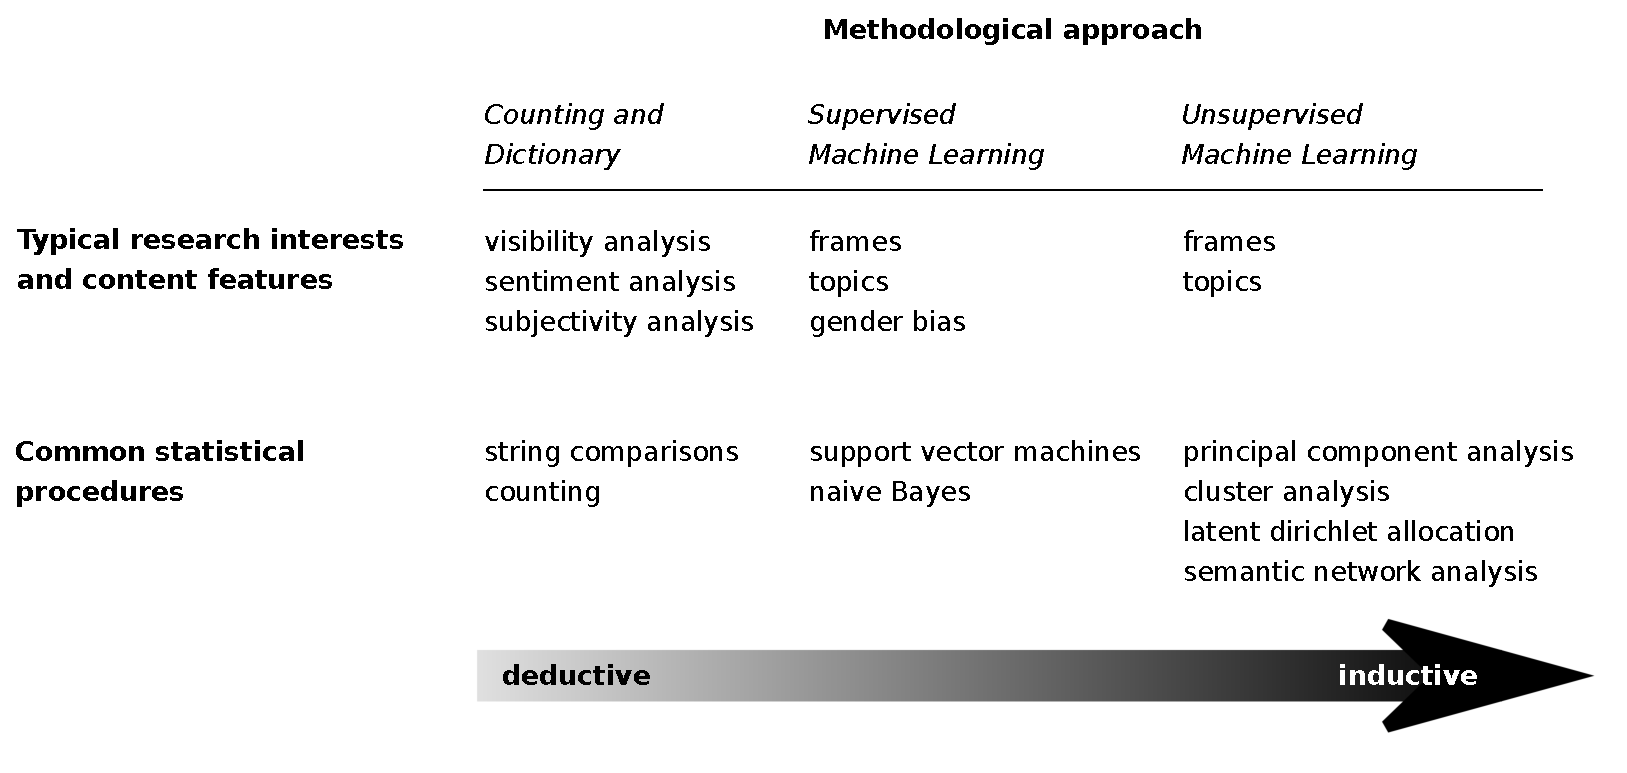
\includegraphics[width=\columnwidth,height=\paperheight,keepaspectratio]{../../pictures/boumanstrilling2016}}
	\\
	\cite{Boumans2016}
\end{frame}





\begin{frame}{Bottom-up vs. top-down}
	\begin{block}{Bottom-up}
	\begin{itemize}
		\item Count most frequently occurring words 
		\item Maybe better: Count combinations of words $\Rightarrow$ Which words co-occur together?
	\end{itemize}
	We \emph{don't} specify what to look for in advance	
	\end{block}
	
	\onslide<2>{
	\begin{block}{Top-down}
	\begin{itemize}
		\item Count frequencies of pre-defined words
		\item Maybe better: patterns instead of words
	\end{itemize}
	We \emph{do} specify what to look for in advance	
\end{block}
}
\end{frame}



\begin{frame}[fragile]{A simple bottom-up approach}
\begin{lstlisting}
from collections import Counter

texts = ["I really really really love him, I do", "I hate him"]

for t in texts:
    print(Counter(t.split()).most_common(3))
\end{lstlisting}
\begin{lstlistingoutput}
[('really', 3), ('I', 2), ('love', 1)]
[('I', 1), ('hate', 1), ('him', 1)]
\end{lstlistingoutput}
\end{frame}




\begin{frame}[fragile]{A simple top-down approach}
\begin{lstlisting}
texts = ["I really really really love him, I do", "I hate him"]
features = ['really', 'love', 'hate']

for t in texts:
    print(f"\nAnalyzing '{t}':")
    for f in features:
        print(f"{f} occurs {t.count(f)} times")
\end{lstlisting}
\begin{lstlistingoutput}
Analyzing 'I really really really love him, I do':
really occurs 3 times
love occurs 1 times
hate occurs 0 times

Analyzing 'I hate him':
really occurs 0 times
love occurs 0 times
hate occurs 1 times

\end{lstlistingoutput}
\end{frame}



\question{When would you use which approach?}




\section{Approaches to working with text}
\subsection{The toolbox}

\begin{frame}{The toolbox}
\begin{block}{Slicing}
\texttt{mystring[2:5]} to get the characters with indices 2,3,4
\end{block}

\begin{block}{String methods}
\begin{itemize}
	\item \texttt{.lower()} returns lowercased string
	\item \texttt{.strip()} returns string without whitespace at beginning and end
	\item \texttt{.find("bla")} returns index of position of substring ``bla'' or -1 if not found
	\item \texttt{.replace("a","b")} returns string where "a" is replaced by "b"
	\item \texttt{.count("bla")} counts how often substring ``bla'' occurs
\end{itemize}
Use tab completion for more!
\end{block}
\end{frame}



\begin{frame}{The toolbox}
\begin{block}{Regular expressions}
(today)
\end{block}


\end{frame}


\subsection{From test to large-scale analysis}

\begin{frame}[fragile]{General approach}
1. Take a single string and test your idea
\begin{lstlisting}
t = "This is a test test test."
print(t.count("test"))
\end{lstlisting}
2a. You'd assume it to return 3. If so, scale it up:
\begin{lstlisting}
results = []
for t in listwithallmytexts:
    r = t.count("test")
    print(f"{t} contains the substring {r} times")
    results.append(r)
\end{lstlisting}

2b. If you \emph{only} need to get the list of results, a list comprehension is more elegant:
\begin{lstlisting}
results = [t.count("test") for t in listwithallmytexts]
\end{lstlisting}


\end{frame}


\begin{frame}[fragile]{General approach}
\Large

\textcolor{red}{Test on a single string, then make a for loop or list comprehension!}

\pause

\normalsize

\begin{alertblock}{Own functions}
If it gets more complex, you can write your own function and then use it in the list comprehension:
\begin{lstlisting}
def mycleanup(t):
   # do sth with string t here, create new string t2
   return t2
  
results = [mycleanup(t) for t in allmytexts]
\end{lstlisting}
\end{alertblock}
\end{frame}


\begin{frame}[fragile]{Pandas string methods as alternative}
If you select column with strings from a pandas dataframe, pandas offers a collection of string methods (via \texttt{.str.}) that largely mirror standard Python string methods:

\begin{lstlisting}
df['newcoloumnwithresults'] = df['columnwithtext'].str.count("bla")
\end{lstlisting} 


\pause

\begin{alertblock}{To pandas or not to pandas for text?}
Partly a matter of taste. 

Not-too-large dataset with a lot of extra columns? Advanced statistical analysis planned? Sounds like pandas.

It's mainly a lot of text? Wanna do some machine learning later on anyway? It's large and (potentially) messy? Doesn't sound like pandas is a good idea.
\end{alertblock}

\end{frame}



\section[Regular expressions]{ACA using regular expressions}

\begin{frame}
	Automated content analysis using regular expressions
\end{frame}



\subsection{What is a regexp?}
\begin{frame}{Regular Expressions: What and why?}
\begin{block}{What is a regexp?}
\begin{itemize}
\item<1-> a \emph{very} widespread way to describe patterns in strings
\item<2-> Think of wildcards like {\tt{*}} or operators like {\tt{OR}}, {\tt{AND}} or {\tt{NOT}} in search strings: a regexp does the same, but is \emph{much} more powerful
\item<3-> You can use them in many editors (!), in the Terminal, in STATA \ldots and in Python
\end{itemize}
\end{block}
\end{frame}

\begin{frame}{An example}
\begin{block}{From last week's task}
\begin{itemize}
\item We wanted to remove everything but words from a tweet
\item We did so by calling the \texttt{.replace()} method
\item We could do this with a regular expression as well: \\
{\tt{ \lbrack \^{}a-zA-Z\rbrack}} would match anything that is not a letter
\end{itemize}
\end{block}
\end{frame}

\begin{frame}{Basic regexp elements}
\begin{block}{Alternatives}
\begin{description}
\item[{\tt{\lbrack TtFf\rbrack}}] matches either T or t or F or f
\item[{\tt{Twitter|Facebook}}] matches either Twitter or Facebook
\item[{\tt{.}}] matches any character
\end{description}
\end{block}
\begin{block}{Repetition}<2->
\begin{description}
\item[{\tt{*}}] the expression before occurs 0 or more times
\item[{\tt{+}}] the expression before occurs 1 or more times
\end{description}
\end{block}
\end{frame}

\begin{frame}{regexp quizz}
\begin{block}{Which words would be matched?}
\tt
\begin{enumerate}
\item<1-> \lbrack Pp\rbrack ython
\item<2-> \lbrack A-Z\rbrack +
\item<3-> RT ?:? @\lbrack a-zA-Z0-9\rbrack *
\end{enumerate}
\end{block}
\end{frame}

\begin{frame}{What else is possible?}
See the table in the book!
\end{frame}

\subsection{Using a regexp in Python}
\begin{frame}{How to use regular expressions in Python}
\begin{block}{The module \texttt{re}*}
\begin{description}
\item<1->[{\tt{re.findall("\lbrack Tt\rbrack witter|\lbrack Ff\rbrack acebook",testo)}}] returns a list with all occurances of Twitter or Facebook in the string called {\tt{testo}}
\item<1->[{\tt{re.findall("\lbrack 0-9\rbrack +\lbrack a-zA-Z\rbrack +",testo)}}] returns a list with all words that start with one or more numbers followed by one or more letters in the string called {\tt{testo}}
\item<2->[{\tt{re.sub("\lbrack Tt\rbrack witter|\lbrack Ff\rbrack acebook","a social medium",testo)}}] returns a string in which all all occurances of Twitter or Facebook are replaced by "a social medium"
\end{description}
\end{block}

\tiny{Use the less-known but more powerful module \texttt{regex} instead to support all dialects used in the book}
\end{frame}


\begin{frame}[fragile]{How to use regular expressions in Python}
\begin{block}{The module re}
\begin{description}
\item<1->[{\tt{re.match(" +(\lbrack 0-9\rbrack +) of (\lbrack 0-9\rbrack +) points",line)}}] returns  \texttt{None} unless it \emph{exactly} matches the string \texttt{line}. If it does, you can access the part between () with the \texttt{.group()} method.
\end{description}
\end{block}

Example:
\begin{lstlisting}
line="             2 of 25 points"
result=re.match(" +([0-9]+) of ([0-9]+) points",line)
if result:
   print ("Your points:",result.group(1))
   print ("Maximum points:",result.group(2))
\end{lstlisting}
Your points: 2\\
Maximum points: 25
\end{frame}














\begin{frame}{Possible applications}
\begin{block}{Data preprocessing}
\begin{itemize}
\item Remove unwanted characters, words, \ldots
\item Identify \emph{meaningful} bits of text: usernames, headlines, where an article starts, \ldots
\item filter (distinguish relevant from irrelevant cases)
\end{itemize}
\end{block}
\end{frame}


\begin{frame}{Possible applications}
\begin{block}{Data analysis: Automated coding}
\begin{itemize}
\item Actors
\item Brands
\item links or other markers that follow a regular pattern
\item Numbers (!)
\end{itemize}
\end{block}
\end{frame}

\begin{frame}[fragile,plain]{Example 1: Counting actors}
\begin{lstlisting}
import re, csv
from glob import glob
count1_list=[]
count2_list=[]
filename_list = glob("/home/damian/articles/*.txt")

for fn in filename_list:
   with open(fn) as fi:
      artikel = fi.read()
      artikel = artikel.replace('\n',' ')
      
      count1 = len(re.findall('Israel.*(minister|politician.*|[Aa]uthorit)',artikel))
      count2 = len(re.findall('[Pp]alest',artikel))

      count1_list.append(count1)
      count2_list.append(count2)
      
output=zip(filename_list,count1_list, count2_list)
with open("results.csv", mode='w',encoding="utf-8") as fo:
    writer = csv.writer(fo)
    writer.writerows(output)
\end{lstlisting}
\end{frame}




\begin{frame}[fragile]{Example 2: Which number has this Lexis Nexis article?}
\begin{lstlisting}
                              All Rights Reserved

                               2 of 200 DOCUMENTS

                                  De Telegraaf

                             21 maart 2014 vrijdag

Brussel bereikt akkoord  aanpak probleembanken;
ECB krijgt meer in melk te brokkelen

SECTION: Finance; Blz. 24
LENGTH: 660 woorden

BRUSSEL   Europa heeft gisteren op de valreep een akkoord bereikt 
over een saneringsfonds voor banken. Daarmee staat de laatste
\end{lstlisting}

\end{frame}

\begin{frame}[fragile]{Example 2: Check the number of a lexis nexis article}
\begin{lstlisting}
                              All Rights Reserved

                               2 of 200 DOCUMENTS

                                  De Telegraaf

                             21 maart 2014 vrijdag

Brussel bereikt akkoord  aanpak probleembanken;
ECB krijgt meer in melk te brokkelen

SECTION: Finance; Blz. 24
LENGTH: 660 woorden

BRUSSEL   Europa heeft gisteren op de valreep een akkoord bereikt 
over een saneringsfonds voor banken. Daarmee staat de laatste
\end{lstlisting}

\begin{lstlisting}
for line in tekst:
    matchObj=re.match(r" +([0-9]+) of ([0-9]+) DOCUMENTS",line)
    if matchObj:
        numberofarticle= int(matchObj.group(1))
        totalnumberofarticles= int(matchObj.group(2))
\end{lstlisting}
\end{frame}


\begin{frame}{Practice yourself!}
	Let's take some time to write some regular expressions.
	Write a script that
\begin{itemize}
	\item extracts URLS form a list of strings
	\item removes everything that is not a letter or number from a list of strings
\end{itemize}
(first develop it for a single string, then scale up)

More tips:
\huge{\url{http://www.pyregex.com/}}
\end{frame}





\begin{frame}{Next meetings}


\begin{block}{Friday}
Write your own ACA script!

Let's take a large dataset on \cite{nelagt2018}.
It's really large and may take some time to download and unpack (1 GB compressed, 10 GB unpacked)!
It can be wise to already download and unpack it, see \url{https://github.com/damian0604/bdaca/blob/master/12ec/week05/exercises/exercise.md}.


\end{block}

\begin{block}{TAKE HOME EXAM}
	Handed out after Friday's meeting\\
	Deadline: Tuesday, 23.59
\end{block}


\end{frame}


\begin{frame}[plain]
	\printbibliography
\end{frame}


\end{document}


